% Ensure that you compile using XeLaTeX !!! PDFTex has problems with some of the packages used
\documentclass[12pt]{article}
\setlength\parindent{0pt}

\usepackage{parskip}
\usepackage[margin=0.5in]{geometry}
\usepackage{fullpage}
\usepackage{moresize}
\usepackage{graphicx}
\usepackage{caption}
\usepackage{subcaption}
\usepackage{float}
\usepackage{xcolor}
\usepackage{soul}
\usepackage{fontspec}
\setmainfont{Doulos SIL}

\begin{document}

\begin{center}
\textbf{{\color{violet}{\HUGE Tuesday, 23 June 2020\\}}}

\textbf{{\color{violet}{\HUGE ALL EXAMS\\}}}

\end{center}
\newpage

\begin{center}
\textbf{{\color{blue}{\HUGE START OF EXAM\\}}}

\textbf{{\color{blue}{\HUGE Student ID: 6745\\}}}

\textbf{{\color{blue}{\HUGE 9:30 - 9:50 AM\\}}}

\end{center}
\newpage

{\large Question 1}\\

Source: Day 9 Handout, Question 1\\

Explain why the concept of an alternation either is or is not useful for understanding this dataset.\\

\begin{figure}[H]
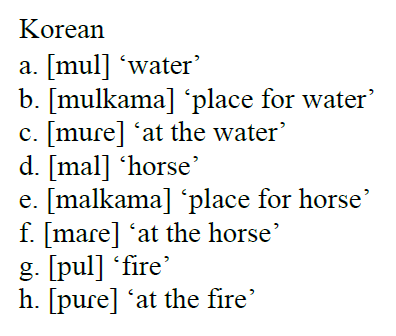
\includegraphics{../images/korean.png}
\end{figure}

\newpage

{\large Question 2}\\

Source: Day 10 Discussion\\

Explain what the given feature’s value is for this class of sounds, and why.\\

{[approximant]}

nasals


\newpage

{\large Question 3}\\

Source: Final Exam Dataset\\

Explain what the underlying representation of these morphemes would be and why.\\

`mix', `past'

\begin{figure}[H]
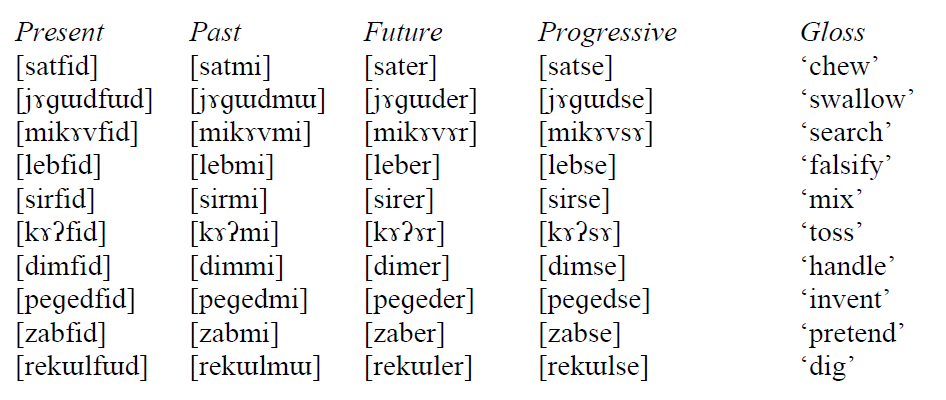
\includegraphics{../images/final_dataset.png}
\end{figure}

\newpage

{\large Question 4}\\

Source: Day 11 Handout, Question 5\\

Explain why this template either does or does not allow syllables of this type to occur.\\

V

\begin{figure}[H]
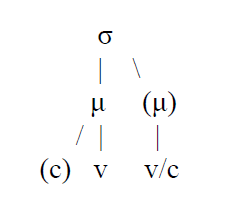
\includegraphics{../images/ponapean_syllabletemplate.png}
\end{figure}

\newpage

{\large Question 5}\\

Source: Day 8 Handout, Question 7\\

Explain why each numbered, underlined statement is true or false. If it is false, explain one way that you could correct it.\\

Sound is an invisible phenomenon. Sound can travel through any substance, $^1$\ul{such as a liquid, solid, or a gas.} $^2$\ul{It involves the transfer of the matter in that substance} from one place to another.\\\\Sound is a particular kind of wave known as $^3$\ul{a compression wave}. $^4$\ul{When the molecules are really close together, we say they are ``rarefied'' and when they are really far apart, we say they are ``compressed.''}


\newpage

{\large Question 6}\\

Source: Day 12 Handout, Question 7\\

Explain how you would figure out the tone-mapping procedures that apply in this dataset.\\

\begin{figure}[H]
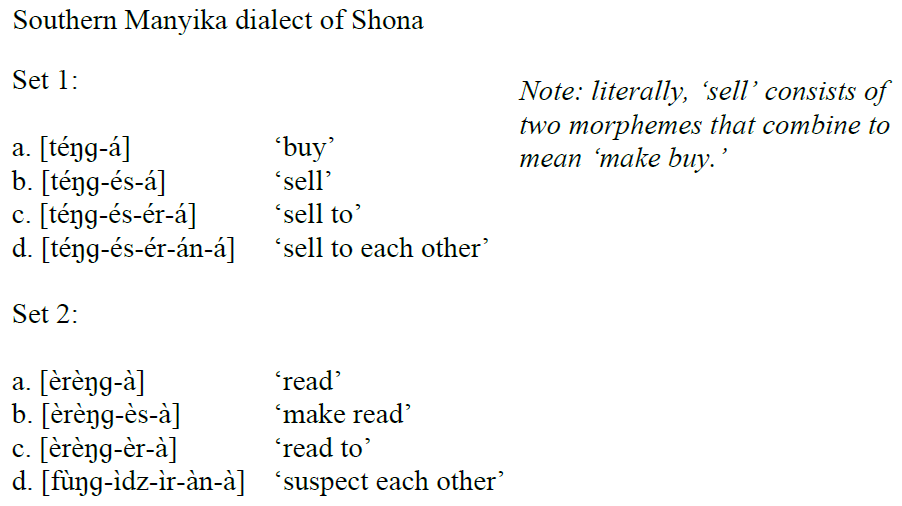
\includegraphics{../images/shona.png}
\end{figure}

\newpage

\begin{center}
\textbf{{\color{red}{\HUGE END OF EXAM}}}\\

\end{center}
\newpage

\begin{center}
\textbf{{\color{blue}{\HUGE START OF EXAM\\}}}

\textbf{{\color{blue}{\HUGE Student ID: 6427\\}}}

\textbf{{\color{blue}{\HUGE 9:50 - 10:10 AM\\}}}

\end{center}
\newpage

{\large Question 1}\\

Source: Day 9 Handout, Question 1\\

Explain why the concept of an alternation either is or is not useful for understanding this dataset.\\

\begin{figure}[H]
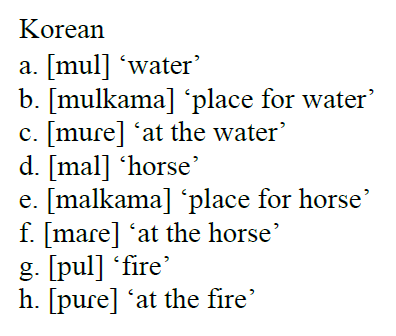
\includegraphics{../images/korean.png}
\end{figure}

\newpage

{\large Question 2}\\

Source: Final Exam Dataset\\

Explain how you would go about figuring out what to analyse in this dataset.\\

\begin{figure}[H]
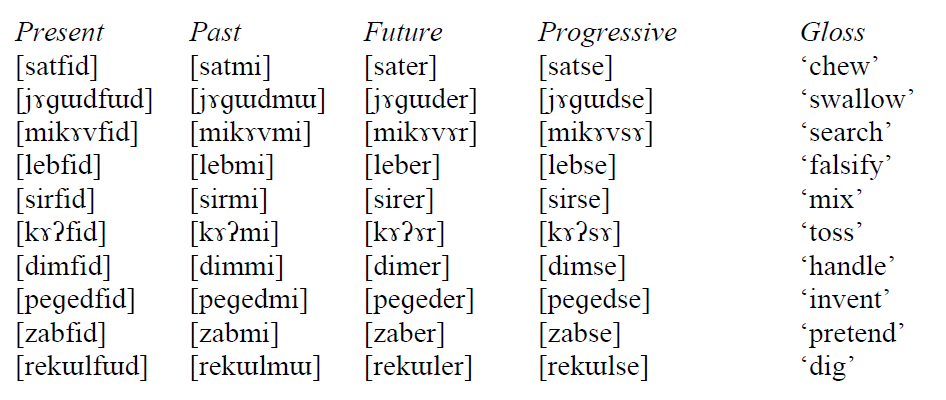
\includegraphics{../images/final_dataset.png}
\end{figure}

\newpage

{\large Question 3}\\

Source: Day 11 Handout, Question 8\\

Explain how you could modify the rule-based approach to take into account the sonority sequencing principle.\\

\begin{figure}[H]
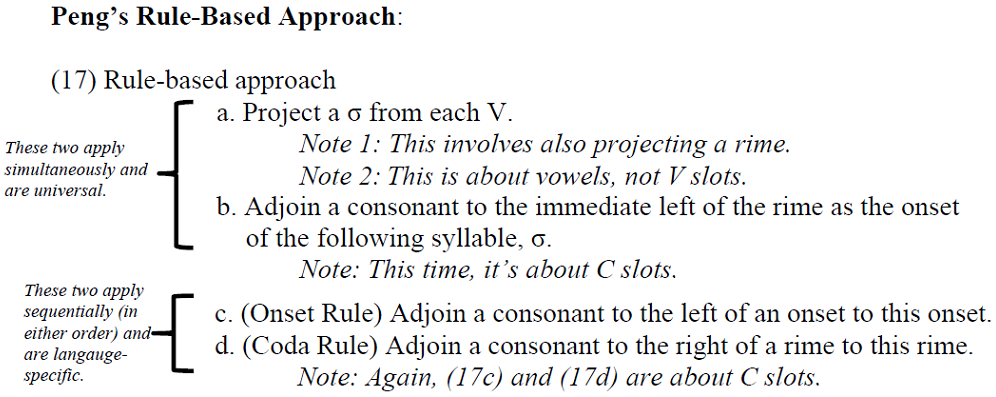
\includegraphics{../images/peng_rules.png}
\end{figure}

\newpage

{\large Question 4}\\

Source: Day 10 Discussion\\

Explain what the given feature’s value is for this class of sounds, and why.\\

{[LABIAL]}

interdentals


\newpage

{\large Question 5}\\

Source: Day 8 Handout, Question 3\\

Explain what you see in the spectrogram that tells you about the properties of the sounds in the pictured word.\\

\begin{figure}[H]
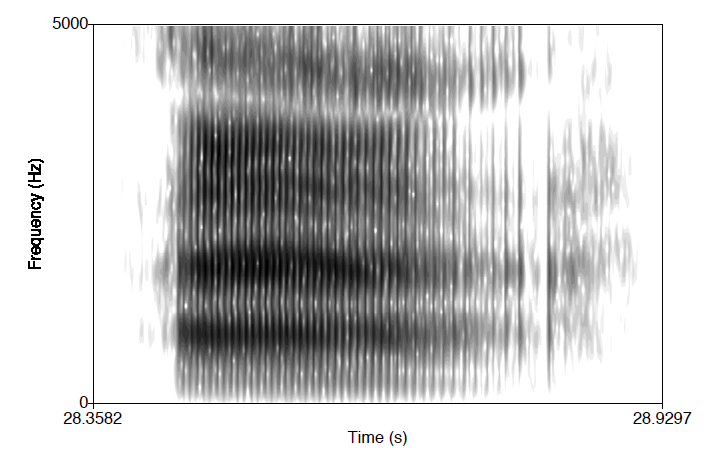
\includegraphics{../images/spectrogram_aaah.png}
\end{figure}

\newpage

{\large Question 6}\\

Source: Quiz 10, Question 3\\

Section 4.2 of chapter 13 in the Peng textbook presented an autosegmental analysis of Mende tone distribution. Explain why the form shown below should NOT be the UR for any morpheme in Mende.\\

\begin{figure}[H]
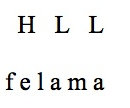
\includegraphics{../images/mende_junction_b.png}
\end{figure}

\newpage

\begin{center}
\textbf{{\color{red}{\HUGE END OF EXAM}}}\\

\end{center}
\newpage

\begin{center}
\textbf{{\color{blue}{\HUGE START OF EXAM\\}}}

\textbf{{\color{blue}{\HUGE Student ID: 3773\\}}}

\textbf{{\color{blue}{\HUGE 10:10 - 10:30 AM\\}}}

\end{center}
\newpage

{\large Question 1}\\

Source: Day 11 Handout, Question 12\\

Explain how understanding syllable structure helps understand the motivation for the process(es) seen in this data.\\

\begin{figure}[H]
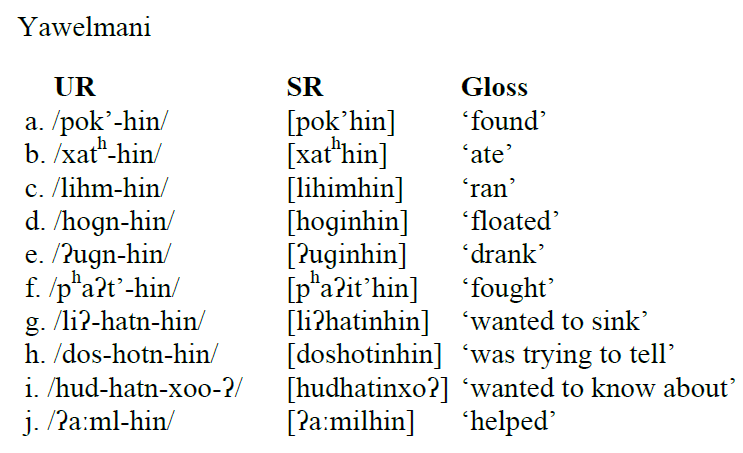
\includegraphics{../images/yawelmani.png}
\end{figure}

\newpage

{\large Question 2}\\

Source: Final Exam Dataset\\

Explain what the underlying representation of these morphemes would be and why.\\

`dig', `future'

\begin{figure}[H]
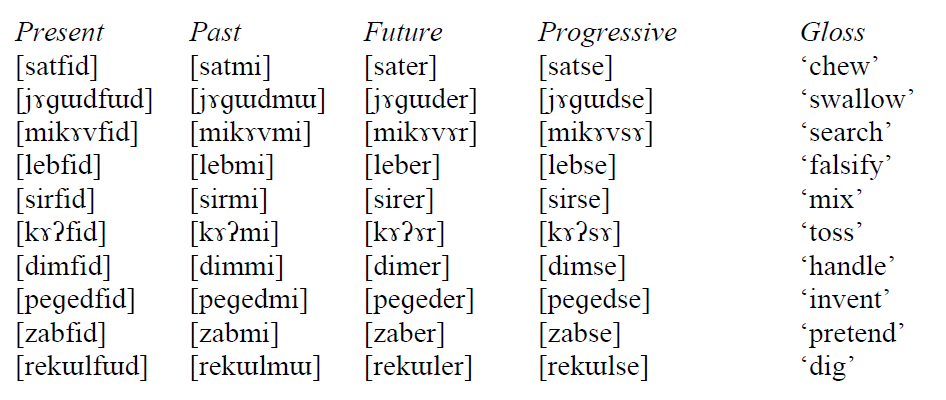
\includegraphics{../images/final_dataset.png}
\end{figure}

\newpage

{\large Question 3}\\

Source: Day 8 Handout, Question 1\\

Explain what (if anything) the letter below represents on this waveform.\\

A

\begin{figure}[H]
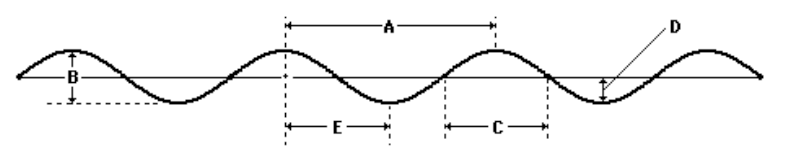
\includegraphics{../images/sinusoid.png}
\end{figure}

\newpage

{\large Question 4}\\

Source: Day 10 Handout, Question 6 (Homework 4, Question 2)\\

Explain how you should use phonological features in this rule. Which parts of the rule should include features, and what features might they be? You don't have to give an exact set of features, but what kinds of features would be involved?\\

/n/ → ∅ / {[m]} \_\_ \#

\begin{figure}[H]
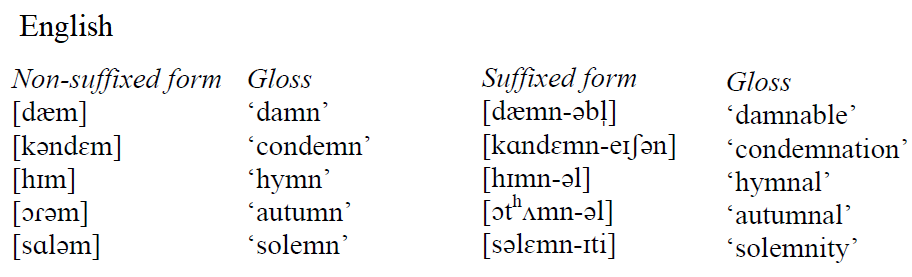
\includegraphics{../images/english_stemalternations.png}
\end{figure}

\newpage

{\large Question 5}\\

Source: Day 9 Handout, Question 4\\

Explain which morpheme(s) in this dataset alternate and how that helps you do a phonological analysis.\\

\begin{figure}[H]
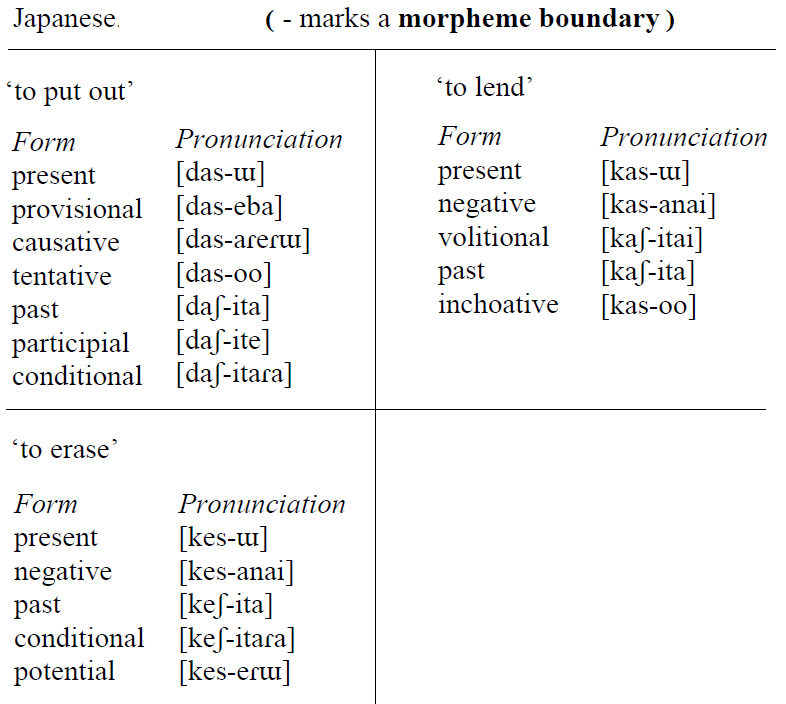
\includegraphics{../images/japanese_verbs.png}
\end{figure}

\newpage

{\large Question 6}\\

Source: Day 12 Handout, Question 6\\

Explain how you would figure out the tone-mapping procedures that apply in this dataset.\\

\begin{figure}[H]
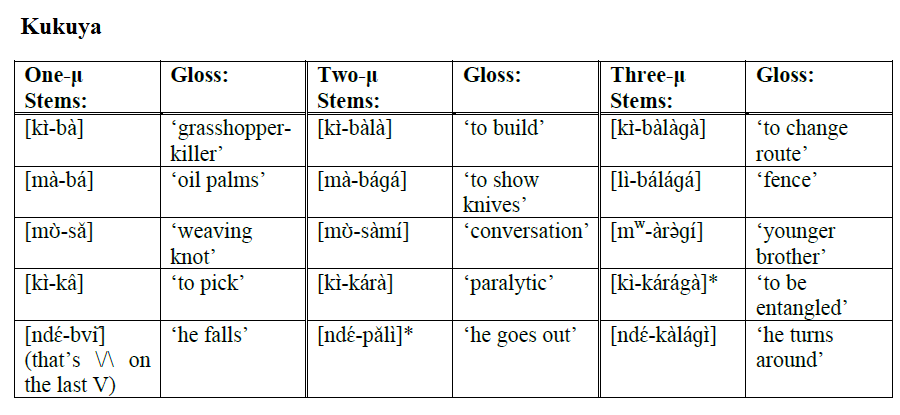
\includegraphics{../images/kukuya.png}
\end{figure}

\newpage

\begin{center}
\textbf{{\color{red}{\HUGE END OF EXAM}}}\\

\end{center}
\newpage

\begin{center}
\textbf{{\color{blue}{\HUGE START OF EXAM\\}}}

\textbf{{\color{blue}{\HUGE Student ID: 9303\\}}}

\textbf{{\color{blue}{\HUGE 10:30 - 10:50 AM\\}}}

\end{center}
\newpage

{\large Question 1}\\

Source: Day 11 Handout, Question 5\\

Explain why this template either does or does not allow syllables of this type to occur.\\

V

\begin{figure}[H]
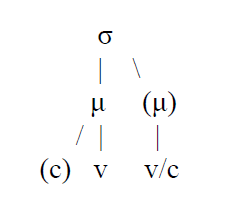
\includegraphics{../images/ponapean_syllabletemplate.png}
\end{figure}

\newpage

{\large Question 2}\\

Source: Final Exam Dataset\\

Explain what the underlying representation of these morphemes would be and why.\\

`dig', `future'

\begin{figure}[H]
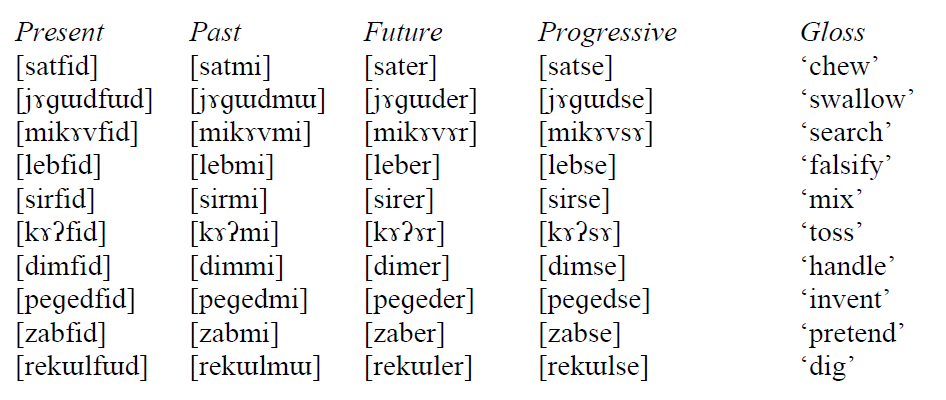
\includegraphics{../images/final_dataset.png}
\end{figure}

\newpage

{\large Question 3}\\

Source: Day 10 Handout, Question 6 (Day 7 Handout, Question 7)\\

Explain how you should use phonological features to combine these rules.\\

/s/ → {[ʃ]} / \_\_ {[i]} \\/z/ → {[dʒ]} / \_\_ {[i]}

\begin{figure}[H]
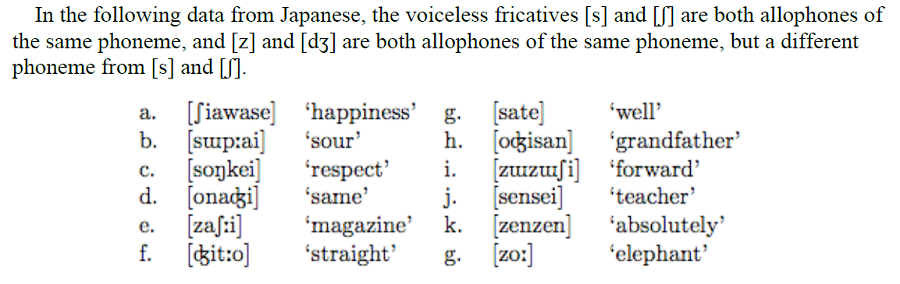
\includegraphics{../images/japanese.png}
\end{figure}

\newpage

{\large Question 4}\\

Source: Day 9 Handout, Question 4\\

Explain which morpheme(s) in this dataset alternate and how that helps you do a phonological analysis.\\

\begin{figure}[H]
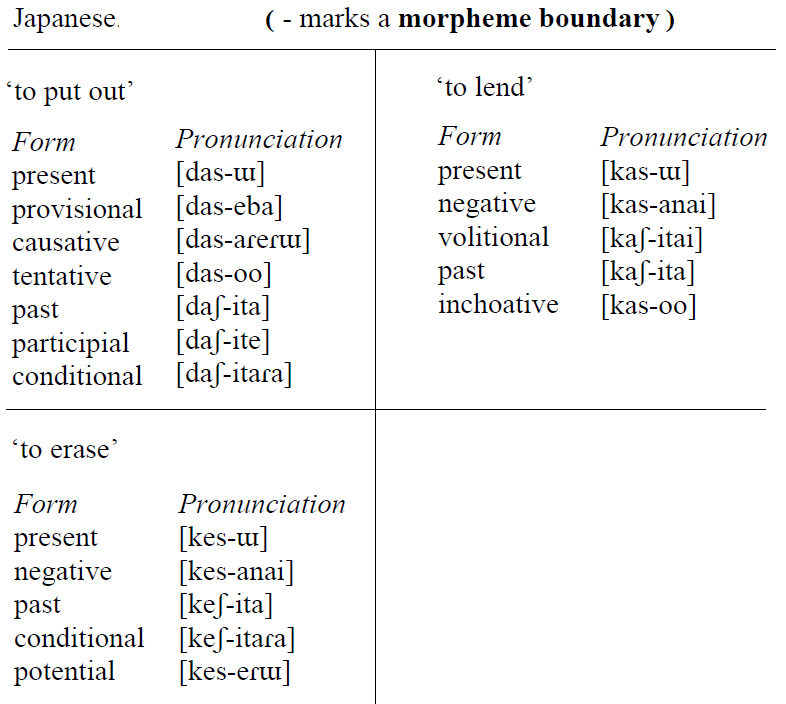
\includegraphics{../images/japanese_verbs.png}
\end{figure}

\newpage

{\large Question 5}\\

Source: Day 8 Handout, Question 1\\

Explain what (if anything) the letter below represents on this waveform.\\

B

\begin{figure}[H]
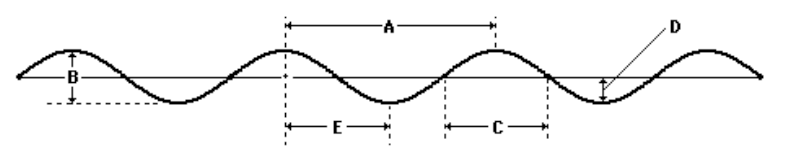
\includegraphics{../images/sinusoid.png}
\end{figure}

\newpage

{\large Question 6}\\

Source: Day 12 Handout, Question 5\\

Explain which of the three rules will apply to the form given below, and whether each of those rules would have an effect or not.\\

Peng’s Tone-Mapping Procedure for Mende: \begin{enumerate} \item L-to-R association: Associate the first tone to the first TBU, the second tone to the second TBU, and so on, until all tones or all TBUS are exhausted. \item Last-TBU Linking: Associate any remaining unlinked tones to the last TBU. \item Last-Tone Linking: Associate the last tone to any TBU without a tone. \end{enumerate}

\begin{figure}[H]
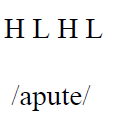
\includegraphics{../images/mendetone_d.png}
\end{figure}

\newpage

\begin{center}
\textbf{{\color{red}{\HUGE END OF EXAM}}}\\

\end{center}
\newpage

\begin{center}
\textbf{{\color{blue}{\HUGE START OF EXAM\\}}}

\textbf{{\color{blue}{\HUGE Student ID: 5824\\}}}

\textbf{{\color{blue}{\HUGE 10:50 - 11:10 AM\\}}}

\end{center}
\newpage

{\large Question 1}\\

Source: Day 11 Handout, Question 5\\

Explain why this template either does or does not allow syllables of this type to occur.\\

CVVC

\begin{figure}[H]
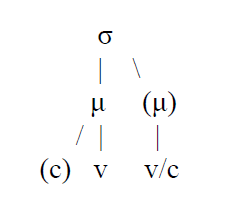
\includegraphics{../images/ponapean_syllabletemplate.png}
\end{figure}

\newpage

{\large Question 2}\\

Source: Final Exam Dataset\\

Explain what the basic phonological analysis of this dataset is, and what the key pieces of evidence are.\\

\begin{figure}[H]
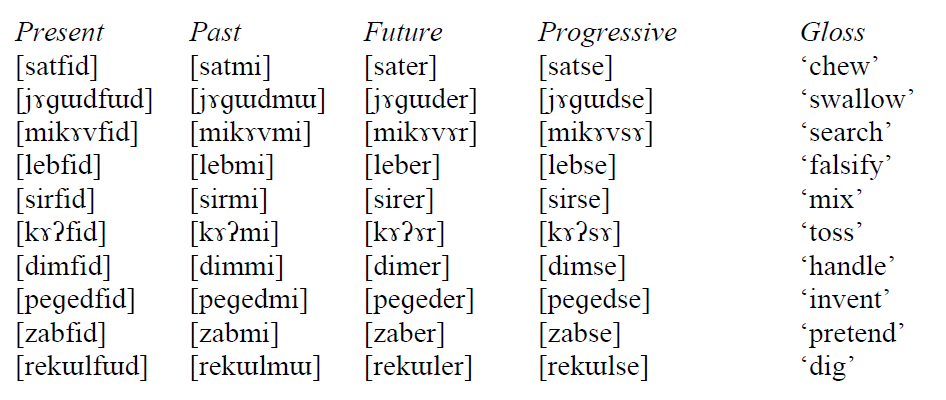
\includegraphics{../images/final_dataset.png}
\end{figure}

\newpage

{\large Question 3}\\

Source: Day 10 Discussion\\

Explain why the given feature's value varies across this set of sounds.\\

{[voice]}

glottalized obstruents


\newpage

{\large Question 4}\\

Source: Day 12 Handout, Question 5\\

Explain which of the three rules will apply to the form given below, and whether each of those rules would have an effect or not.\\

Peng’s Tone-Mapping Procedure for Mende: \begin{enumerate} \item L-to-R association: Associate the first tone to the first TBU, the second tone to the second TBU, and so on, until all tones or all TBUS are exhausted. \item Last-TBU Linking: Associate any remaining unlinked tones to the last TBU. \item Last-Tone Linking: Associate the last tone to any TBU without a tone. \end{enumerate}

\begin{figure}[H]
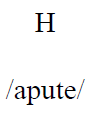
\includegraphics{../images/mendetone_b.png}
\end{figure}

\newpage

{\large Question 5}\\

Source: Day 8 Handout, Question 3\\

Explain what you see in the spectrogram that tells you about the properties of the sounds in the pictured word.\\

\begin{figure}[H]
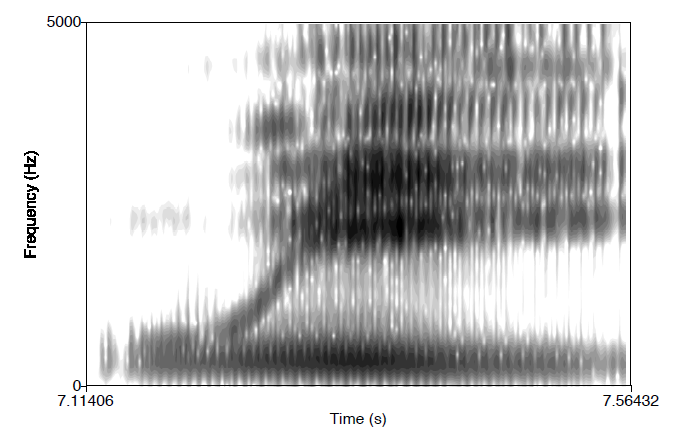
\includegraphics{../images/spectrogram_we.png}
\end{figure}

\newpage

{\large Question 6}\\

Source: Day 9 Handout, Question 3\\

Explain which morpheme(s) in this dataset alternate and how that helps you do a phonological analysis.\\

\begin{figure}[H]
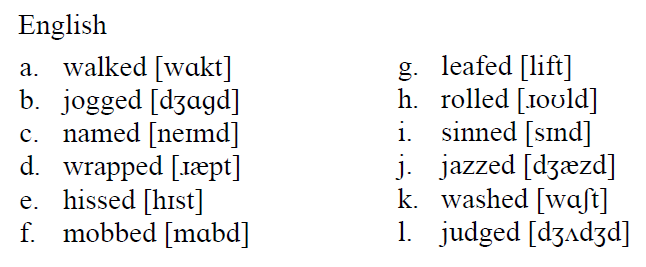
\includegraphics{../images/english_past.png}
\end{figure}

\newpage

\begin{center}
\textbf{{\color{red}{\HUGE END OF EXAM}}}\\

\end{center}
\newpage

\begin{center}
\textbf{{\color{blue}{\HUGE START OF EXAM\\}}}

\textbf{{\color{blue}{\HUGE Student ID: 5540\\}}}

\textbf{{\color{blue}{\HUGE 11:10 - 11:30 AM\\}}}

\end{center}
\newpage

{\large Question 1}\\

Source: Day 11 Handout, Question 13\\

Explain how understanding syllable structure helps understand the motivation for the process(es) seen in this data.\\

\begin{figure}[H]
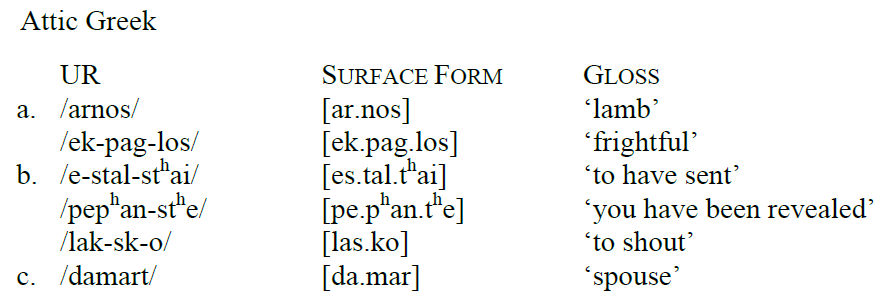
\includegraphics{../images/atticgreek.png}
\end{figure}

\newpage

{\large Question 2}\\

Source: Final Exam Dataset\\

Explain what the underlying representation of these morphemes would be and why.\\

`mix', `past'

\begin{figure}[H]
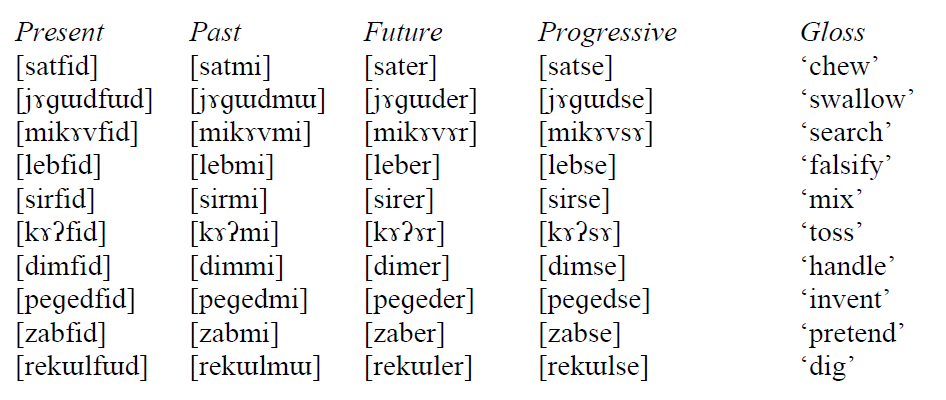
\includegraphics{../images/final_dataset.png}
\end{figure}

\newpage

{\large Question 3}\\

Source: Day 8 Handout, Question 3\\

Explain what you see in the spectrogram that tells you about the properties of the sounds in the pictured word.\\

\begin{figure}[H]
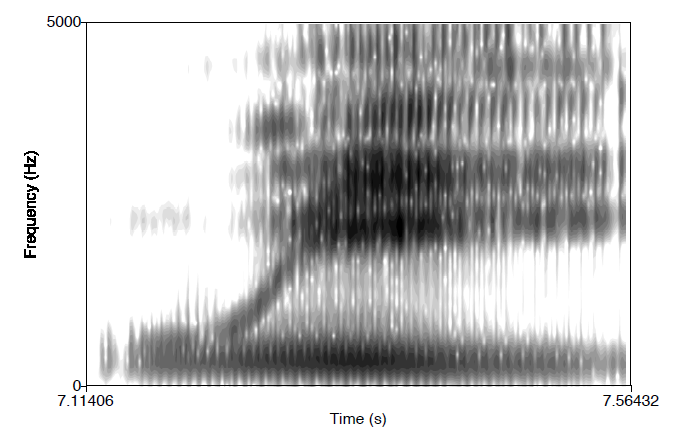
\includegraphics{../images/spectrogram_we.png}
\end{figure}

\newpage

{\large Question 4}\\

Source: Day 12 Handout, Question 6\\

Explain how you would figure out the tone-mapping procedures that apply in this dataset.\\

\begin{figure}[H]
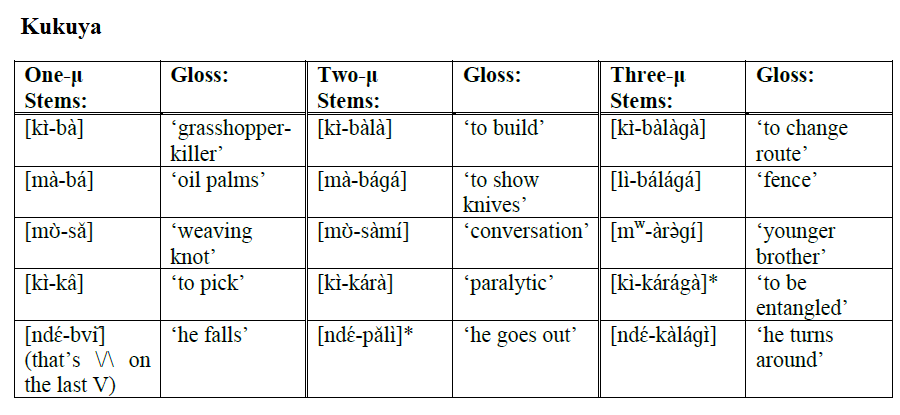
\includegraphics{../images/kukuya.png}
\end{figure}

\newpage

{\large Question 5}\\

Source: Quiz 8, Question 3\\

Explain why this featural specification either does or does not match the given sound.\\

{[+consonantal]}, {[+sonorant]}

{[m]}


\newpage

{\large Question 6}\\

Source: Day 9 Handout, Question 3\\

Explain which morpheme(s) in this dataset alternate and how that helps you do a phonological analysis.\\

\begin{figure}[H]
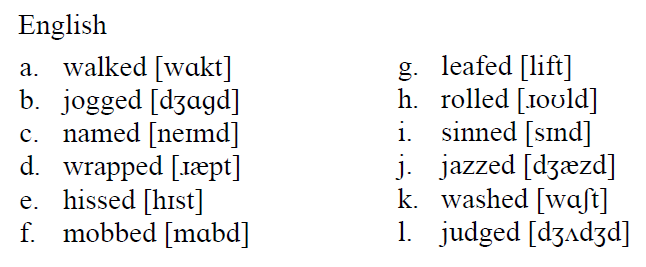
\includegraphics{../images/english_past.png}
\end{figure}

\newpage

\begin{center}
\textbf{{\color{red}{\HUGE END OF EXAM}}}\\

\end{center}
\newpage

\begin{center}
\textbf{{\color{blue}{\HUGE START OF EXAM\\}}}

\textbf{{\color{blue}{\HUGE Student ID: 1887\\}}}

\textbf{{\color{blue}{\HUGE 11:30 - 11:50 AM\\}}}

\end{center}
\newpage

{\large Question 1}\\

Source: Day 9 Handout, Question 2\\

Explain why the concept of an alternation either is or is not useful for understanding this dataset.\\

\begin{figure}[H]
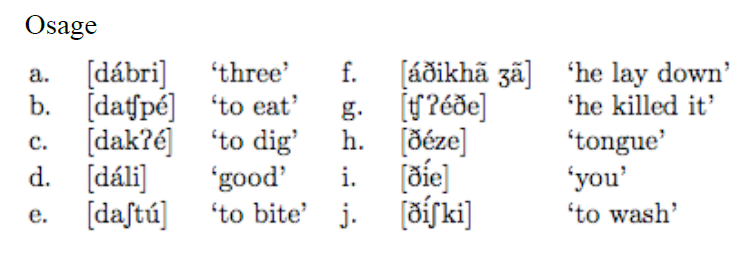
\includegraphics{../images/osage.png}
\end{figure}

\newpage

{\large Question 2}\\

Source: Final Exam Dataset\\

Explain what the underlying representation of these morphemes would be and why.\\

`invent', `progressive'

\begin{figure}[H]
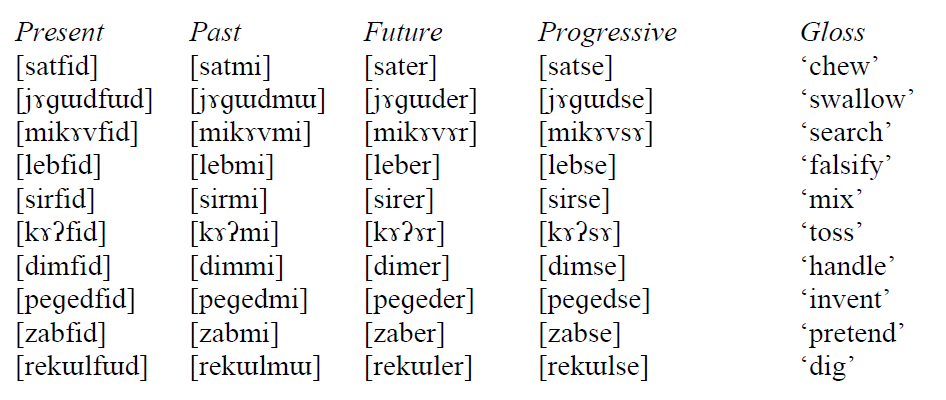
\includegraphics{../images/final_dataset.png}
\end{figure}

\newpage

{\large Question 3}\\

Source: Day 8 Handout, Question 7\\

Explain why each numbered, underlined statement is true or false. If it is false, explain one way that you could correct it.\\

We can visualize speech through the use of spectra and spectrograms. $^{18}$\ul{A spectrogram shows frequency on the horizontal axis and amplitude on the vertical axis.} $^{19}$\ul{A spectrum, on the other hand, shows frequency on the vertical axis and time along the horizontal axis}.\\\\$^{20}$\ul{On a spectrogram, the dark bars are called formants.} $^{21}$\ul{The formants correspond to the amplitude peaks on a spectrum.}


\newpage

{\large Question 4}\\

Source: Quiz 10, Question 1\\

Section 4.2 of chapter 13 in the Peng textbook presented an autosegmental analysis of Mende tone distribution. Explain why the form shown below should NOT be the UR for any morpheme in Mende.\\

\begin{figure}[H]
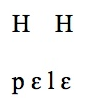
\includegraphics{../images/mende_house_b.png}
\end{figure}

\newpage

{\large Question 5}\\

Source: Homework 5, Question 1\\

Explain which sound should be removed to make this a natural class, and what the minimum set of features would be to describe the resulting natural class.\\

{[v]}, {[z]}, {[ʃ]}, {[ʒ]}, {[ð]}


\newpage

{\large Question 6}\\

Source: Quiz 9, Question 12\\

Explain the key differences between the templatic and the rule-based approaches to syllabification.\\


\newpage

\begin{center}
\textbf{{\color{red}{\HUGE END OF EXAM}}}\\

\end{center}
\newpage

\begin{center}
\textbf{{\color{blue}{\HUGE START OF EXAM\\}}}

\textbf{{\color{blue}{\HUGE Student ID: 4199\\}}}

\textbf{{\color{blue}{\HUGE 11:50 AM - 12:10 PM\\}}}

\end{center}
\newpage

{\large Question 1}\\

Source: Day 9 Handout, Question 1\\

Explain why the concept of an alternation either is or is not useful for understanding this dataset.\\

\begin{figure}[H]
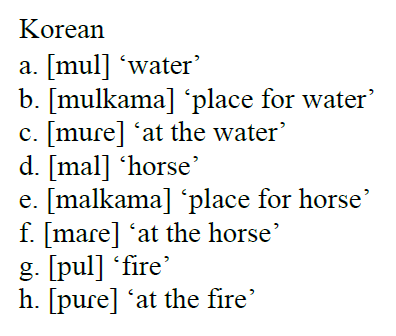
\includegraphics{../images/korean.png}
\end{figure}

\newpage

{\large Question 2}\\

Source: Day 8 Handout, Question 4\\

Explain how each component of the description below gives you information about the sound being described.\\

This consonant is characterized by having a lot of random noise in the spectrogram, with no clear formant structure at all. It tends to be longer and louder than other similar consonants. There is no voice bar, and the majority of the noise created by this consonant is at relatively high frequencies.


\newpage

{\large Question 3}\\

Source: Final Exam Dataset\\

Explain how you would go about figuring out what to analyse in this dataset.\\

\begin{figure}[H]
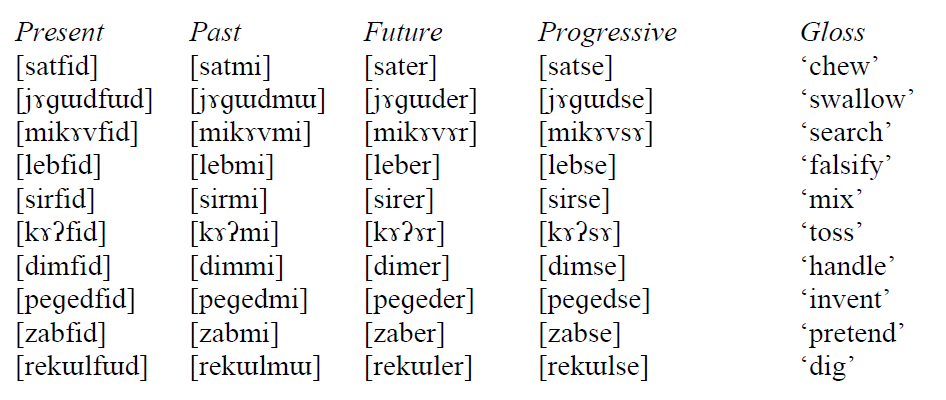
\includegraphics{../images/final_dataset.png}
\end{figure}

\newpage

{\large Question 4}\\

Source: Homework 5, Question 1\\

Explain which sound should be removed to make this a natural class, and what the minimum set of features would be to describe the resulting natural class.\\

{[i]}, {[ɪ]}, {[ɛ]}, {[u]}, {[ʊ]}


\newpage

{\large Question 5}\\

Source: Day 11 Handout, Question 5\\

Explain why this template either does or does not allow syllables of this type to occur.\\

VCC

\begin{figure}[H]
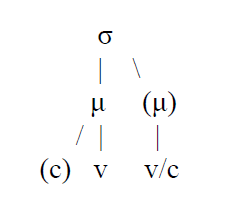
\includegraphics{../images/ponapean_syllabletemplate.png}
\end{figure}

\newpage

{\large Question 6}\\

Source: Day 12 Handout, Question 7\\

Explain how you would figure out the underlying representations of the suffix morphemes in this dataset.\\

\begin{figure}[H]
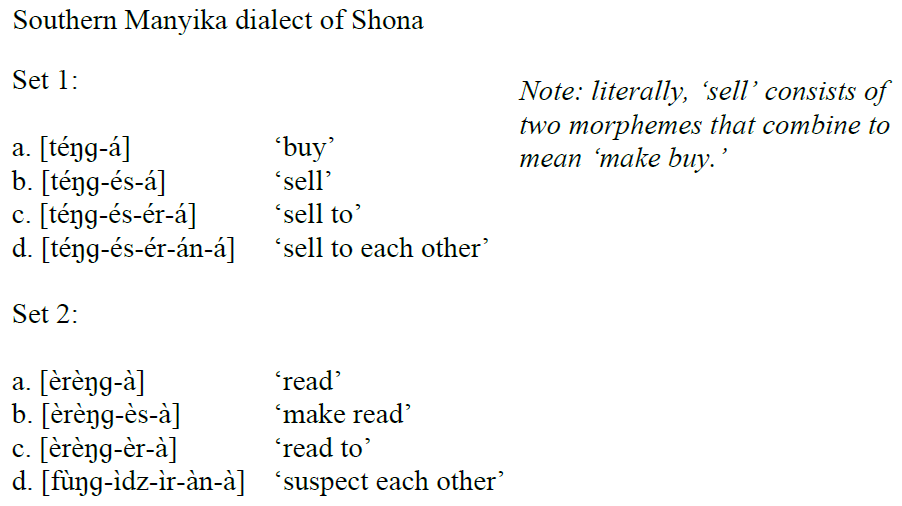
\includegraphics{../images/shona.png}
\end{figure}

\newpage

\begin{center}
\textbf{{\color{red}{\HUGE END OF EXAM}}}\\

\end{center}
\newpage

\begin{center}
\textbf{{\color{blue}{\HUGE START OF EXAM\\}}}

\textbf{{\color{blue}{\HUGE Student ID: 1794\\}}}

\textbf{{\color{blue}{\HUGE 12:10 - 12:30 PM\\}}}

\end{center}
\newpage

{\large Question 1}\\

Source: Day 11 Handout, Question 12\\

Explain how understanding syllable structure helps understand the motivation for the process(es) seen in this data.\\

\begin{figure}[H]
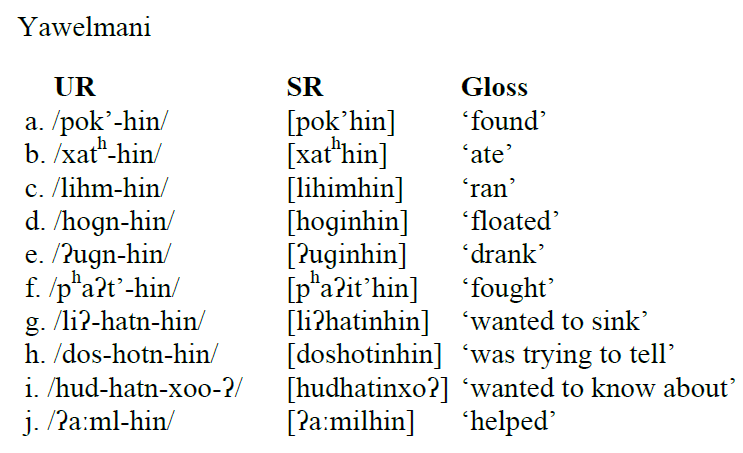
\includegraphics{../images/yawelmani.png}
\end{figure}

\newpage

{\large Question 2}\\

Source: Day 10 Discussion\\

Explain what the given feature’s value is for this class of sounds, and why.\\

{[strident]}

glides


\newpage

{\large Question 3}\\

Source: Final Exam Dataset\\

Explain what the underlying representation of these morphemes would be and why.\\

`mix', `past'

\begin{figure}[H]
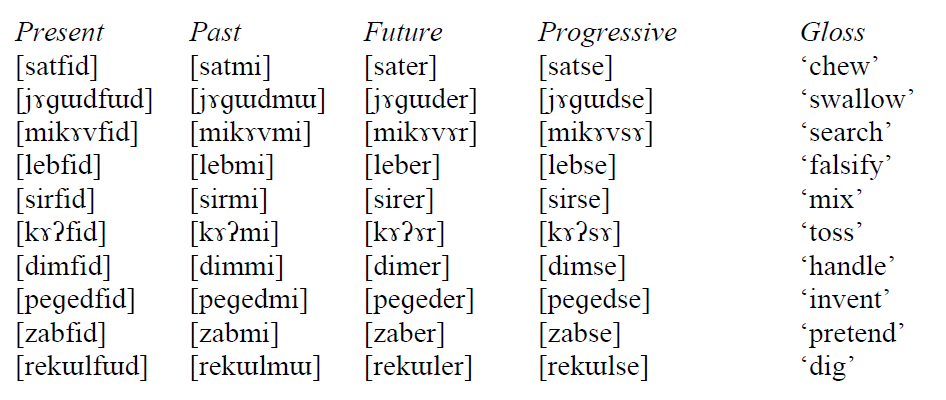
\includegraphics{../images/final_dataset.png}
\end{figure}

\newpage

{\large Question 4}\\

Source: Day 12 Handout, Question 5\\

Explain which of the three rules will apply to the form given below, and whether each of those rules would have an effect or not.\\

Peng’s Tone-Mapping Procedure for Mende: \begin{enumerate} \item L-to-R association: Associate the first tone to the first TBU, the second tone to the second TBU, and so on, until all tones or all TBUS are exhausted. \item Last-TBU Linking: Associate any remaining unlinked tones to the last TBU. \item Last-Tone Linking: Associate the last tone to any TBU without a tone. \end{enumerate}

\begin{figure}[H]
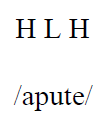
\includegraphics{../images/mendetone_a.png}
\end{figure}

\newpage

{\large Question 5}\\

Source: Day 9 Handout, Question 5\\

Explain which morpheme(s) in this dataset alternate and how that helps you do a phonological analysis.\\

\begin{figure}[H]
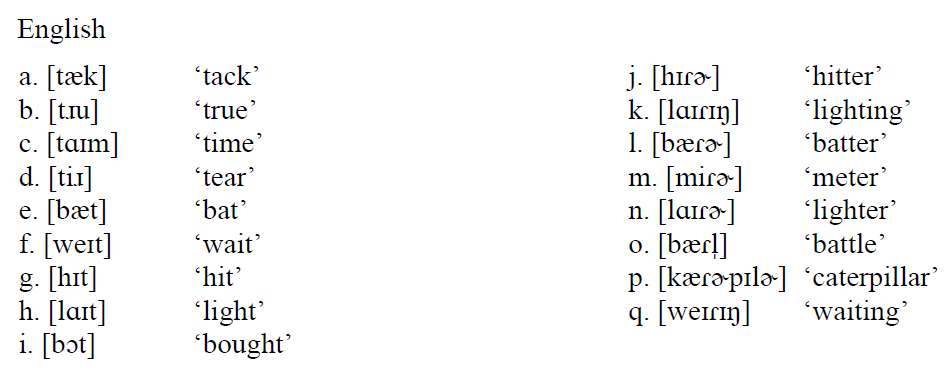
\includegraphics{../images/english_t_flap.png}
\end{figure}

\newpage

{\large Question 6}\\

Source: Day 8 Handout, Question 3\\

Explain what you see in the spectrogram that tells you about the properties of the sounds in the pictured word.\\

\begin{figure}[H]
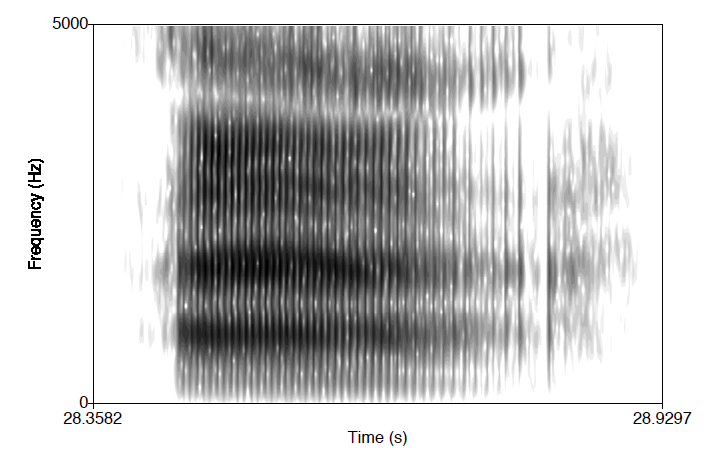
\includegraphics{../images/spectrogram_aaah.png}
\end{figure}

\newpage

\begin{center}
\textbf{{\color{red}{\HUGE END OF EXAM}}}\\

\end{center}
\newpage

\begin{center}
\textbf{{\color{blue}{\HUGE START OF EXAM\\}}}

\textbf{{\color{blue}{\HUGE Student ID: 4656\\}}}

\textbf{{\color{blue}{\HUGE 12:30 - 12:50 PM\\}}}

\end{center}
\newpage

{\large Question 1}\\

Source: Day 11 Handout, Question 10\\

Explain why this structure either is or is not a correct application of the templatic-based approach to syllabification, using the provided template and assuming that syllabification proceeds from left to right.\\

\begin{figure}[H]
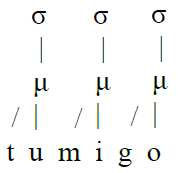
\includegraphics{../images/pengtemplate_tumigo_yes.png}
\end{figure}
\begin{figure}[H]
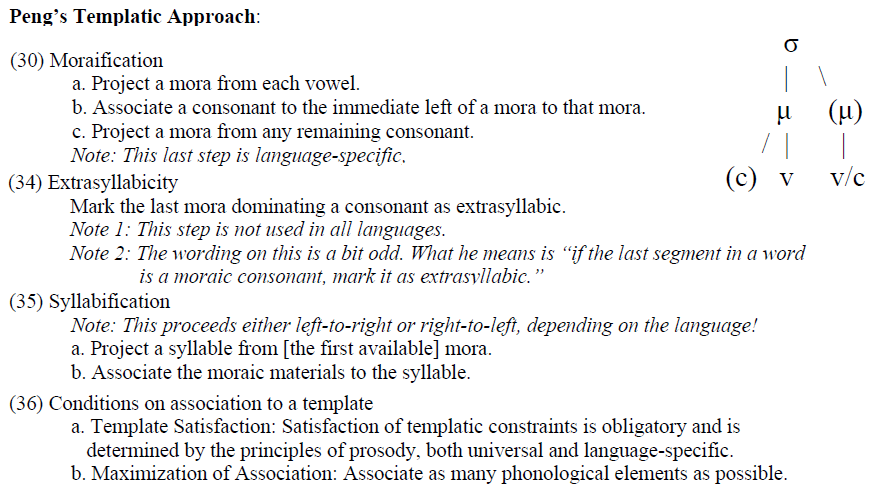
\includegraphics{../images/peng_template_withdiagram.png}
\end{figure}

\newpage

{\large Question 2}\\

Source: Day 10 Handout, Question 5\\

Explain why you either should or should not use phonological features in the CONTEXT of the given rule.\\

Vowel laxing: /i/ → {[ɪ]} / \{{[ɛ]}, {[ɔ]}\} C$_0$\_\_


\newpage

{\large Question 3}\\

Source: Final Exam Dataset\\

Explain how you would go about figuring out what to analyse in this dataset.\\

\begin{figure}[H]
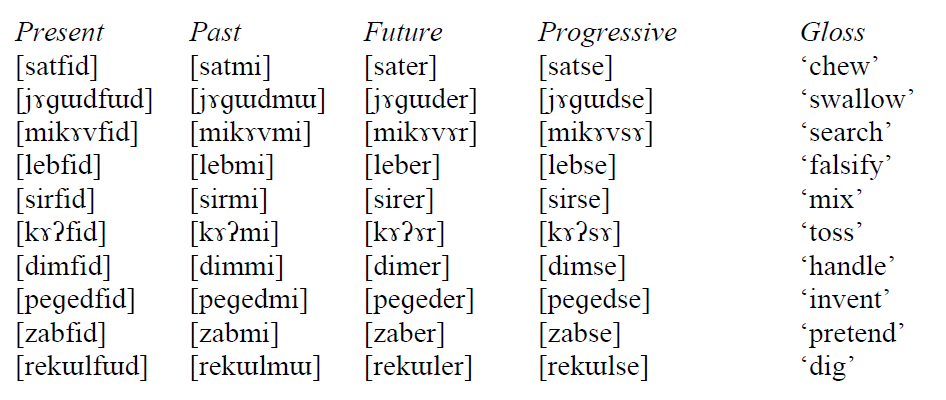
\includegraphics{../images/final_dataset.png}
\end{figure}

\newpage

{\large Question 4}\\

Source: Quiz 7, Question 8\\

Based on this data from Lamba, explain why the pair given below either does or does not show that the consonants preceding the morpheme for `with' are NOT responsible for the variation between [-il] and [-el].\\

tul-il-a \& soŋk-el-a

\begin{figure}[H]
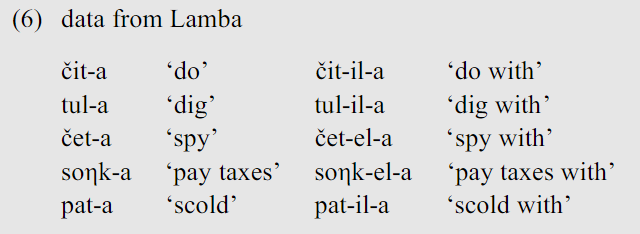
\includegraphics{../images/peng119_lamba.png}
\end{figure}

\newpage

{\large Question 5}\\

Source: Day 8 Handout, Question 3\\

Explain what you see in the spectrogram that tells you about the properties of the sounds in the pictured word.\\

\begin{figure}[H]
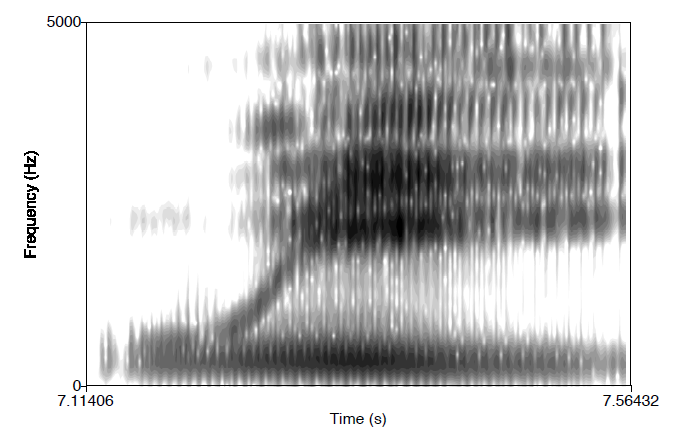
\includegraphics{../images/spectrogram_we.png}
\end{figure}

\newpage

{\large Question 6}\\

Source: Day 12 Handout, Question 5\\

Explain which of the three rules will apply to the form given below, and whether each of those rules would have an effect or not.\\

Peng’s Tone-Mapping Procedure for Mende: \begin{enumerate} \item L-to-R association: Associate the first tone to the first TBU, the second tone to the second TBU, and so on, until all tones or all TBUS are exhausted. \item Last-TBU Linking: Associate any remaining unlinked tones to the last TBU. \item Last-Tone Linking: Associate the last tone to any TBU without a tone. \end{enumerate}

\begin{figure}[H]
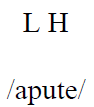
\includegraphics{../images/mendetone_c.png}
\end{figure}

\newpage

\begin{center}
\textbf{{\color{red}{\HUGE END OF EXAM}}}\\

\end{center}
\newpage

\begin{center}
\textbf{{\color{blue}{\HUGE START OF EXAM\\}}}

\textbf{{\color{blue}{\HUGE Student ID: 8079\\}}}

\textbf{{\color{blue}{\HUGE 12:50 - 1:10 PM\\}}}

\end{center}
\newpage

{\large Question 1}\\

Source: Day 8 Handout, Question 1\\

Explain what (if anything) the letter below represents on this waveform.\\

C

\begin{figure}[H]
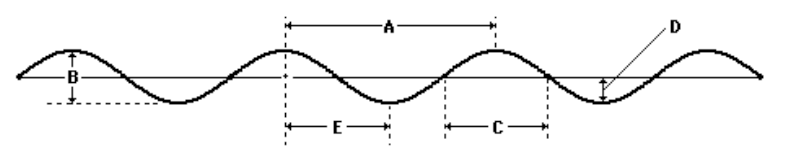
\includegraphics{../images/sinusoid.png}
\end{figure}

\newpage

{\large Question 2}\\

Source: Quiz 8, Question 3\\

Explain why this featural specification either does or does not match the given sound.\\

{[-consonantal]}, {[-sonorant]}

{[u]}


\newpage

{\large Question 3}\\

Source: Final Exam Dataset\\

Explain what rule or rules would apply in this dataset and how you know.\\

\begin{figure}[H]
\includegraphics{../images/final_dataset.png}
\end{figure}

\newpage

{\large Question 4}\\

Source: Day 9 Handout, Question 3\\

Explain which morpheme(s) in this dataset alternate and how that helps you do a phonological analysis.\\

\begin{figure}[H]
\includegraphics{../images/english_past.png}
\end{figure}

\newpage

{\large Question 5}\\

Source: Day 12 Handout, Question 6\\

Explain how you would figure out the tone-mapping procedures that apply in this dataset.\\

\begin{figure}[H]
\includegraphics{../images/kukuya.png}
\end{figure}

\newpage

{\large Question 6}\\

Source: Homework 5, Question 2\\

Explain why the insertion analysis is better than the deletion analysis for this dataset.\\

\begin{figure}[H]
\includegraphics{../images/fula.png}
\end{figure}

\newpage

\begin{center}
\textbf{{\color{red}{\HUGE END OF EXAM}}}\\

\end{center}
\newpage

\end{document}

